\selectlanguage{ngerman}%
\frenchspacing%
\begin{ledgroupsized}[r]{120mm}%
\footnotesize%
\pstart%
\noindent\textbf{Überlieferung:}%
\pend%
\end{ledgroupsized}%
\begin{ledgroupsized}[r]{114mm}%
\footnotesize%
\pstart%
\parindent -6mm%
\makebox[6mm][l]{\textit{L}}%
Aufzeichnung:
LH XXXVII 4, Bl.\,159.
Ein Blatt 4\textsuperscript{o};
\href{\Scan{LH_37_04_159_wz}}{Wasserzeichen} mittig; %
Ränder beschnitten;
Papiererhaltungsmaßnahmen.
Zwei ganzseitig beschriebene Seiten.
\pend%
\end{ledgroupsized}%
\selectlanguage{latin}%
\frenchspacing%
\vspace{5mm}%
\normalsize%
\pstart%
\noindent%
\lbrack%
\href{\Scan{LH_37_04_159r}}%
{159\,r\textsuperscript{o}}%
\rbrack
\phantom{12 November 1677}%
\hfill%
\phantom{\lbrack159\,r\textsuperscript{o}\rbrack}%
12 Novembris 1677%
\pend%
\pstart%
\noindent%
\centering%
De Barometro portabili%
\indexS{barometrum portabile}%
\\
Scheda 2%
\indexS{scheda}%
\edlabel{LH_37_04_159_159r_sjg-1}%
\edtext{}{%
\xxref{LH_37_04_159_159r_sjg-1}{LH_37_04_159_159r_sjg-2}%
\lemma{Scheda 2}%
\Bfootnote{%
\lbrack/\rbrack\ %
\textit{(1)}~Sit instrumentum vitreum \textit{ABCDEFGH} apertum in \textit{G} et \textit{H}. \textit{BCD} sit liquor. Calefiat quantum licet phiala vitrea \textit{E}, %
\textit{(a)}~\bars{aere \textit{erg.}} pelletur liquor infra \textit{D} super \textit{B} ex parte, et ex alia parte expelletur per %
\textit{(b)}~\bars{et \textit{erg.}} aer in \textit{E} partim pelletur versus \textit{D}, deprimetque liquorem infra \textit{D}, eriget supra \textit{B}, partim expelletur per \textit{G} (expellendo aerem in \textit{A} ex \textit{H}) %
\textit{(c)}~partim aer in \textit{E} pelletur versus %
\lbrack/\rbrack\ %
\textit{(2)}~Sit instrumentum %
\lbrack...\rbrack\ in \textit{A}, \textit{E}, %
\bars{\textit{L} \textit{ändert Hrsg.}}. Infuso per \textit{A} %
\lbrack...\rbrack\ Hermetice exitus \textit{E} %
\textit{(a)}~et pila~\textit{E} %
\textit{(b)}~(qui tubulus %
\lbrack...\rbrack\ pila \textit{E} fortissime %
\textit{(aa)}~igne %
\textit{(bb)}~incalescat, ita %
\lbrack...\rbrack\ Quo facto %
\textit{(aaa)}~contingeat %
\textit{(bbb)}~aer %
\textit{(aaaa)}~in %
\textit{(bbbb)}~ex pila \textit{E} %
\lbrack...\rbrack\ infra \textit{D} %
\bars{in \textit{d} \textit{erg.}}, et eriget supra \textit{B} %
\bars{in \textit{b} \textit{erg.}}, et aerem aliquem %
\textit{(aaaaa)}~per \textit{A} %
\textit{(bbbbb)}~inter \textit{A} et \textit{B} %
\lbrack...\rbrack\ per \textit{H} effluere faciet.%
~\textit{L}%
}}%
\pend%
\vspace{0.5em}%
\pstart%
\noindent%
\lbrack%
\textit{Nachfolgend kleingedruckter Text gestrichen:}%
\rbrack%
\pend%
\vspace{0.5em}%
\footnotesize%
\pstart%
\noindent%
Sit instrumentum vitreum \textit{ABCDEFGH}%
\indexS{instrumentum vitreum}
apertum in \textit{A}, \textit{E}, \lbrack\textit{H}\rbrack.
Infuso per \textit{A} liquore impleatur \textit{BCD}.%
\indexS{liquor infusus barometro}
Infuso per \textit{H} liquore impleatur \textit{HGF}.
Sigilletur Hermetice exitus \textit{E}%
\indexS{exitus sigillatus hermetice}
(qui tubulus%
\indexS{tubulus vitreus}
esse potest%
\lbrack)\rbrack\
et pila~\textit{E}%
\indexS{pila barometri}
fortissime incalescat,%
\indexS{pila incalescens}
ita tamen ut ne fundatur.
Quo facto
aer ex pila \textit{E} expulsus%
\indexS{aer expulsus e barometro}
partim tendens versus~\textit{D}
liquorem premet infra \textit{D}
in \textit{d},
et eriget supra \textit{B}
in \textit{b},
et aerem aliquem
inter \textit{A} et \textit{B} positum
per \textit{A} expellet;%
\indexS{aer expulsus e barometro}
partim tendens versus \textit{F}
liquorem deprimet infra \textit{F},%
\indexS{liquor infusus barometro}
et erigens supra \textit{H} expellet%
\indexS{liquor expulsus e barometro}
seu per \textit{H} effluere faciet.%
\edlabel{LH_37_04_159_159r_sjg-2}
His factis
\edtext{%
claudatur exitus%
\indexS{exitus clausus}%
}{%
\lemma{claudatur}%
\Bfootnote{%
\textit{(1)}~foramen %
\textit{(2)}~exitus%
~\textit{L}%
}}
\textit{A}
(qui tubulus%
\indexS{tubulus vitreus}
esse potest%
\lbrack)\rbrack\
et refrigerata jam machina paulatim%
\indexS{machina refrigerata}%
\indexS{refrigeratio machinae}
duo aequali vi%
\indexS{vis aequalis}%
\indexS{vis aeris ambientis}%
\indexS{vis aeris ordinarii}
\edtext{%
agent in aerem%
}{%
\lemma{agent in}%
\Bfootnote{%
\textit{(1)}~aquam %
\textit{(2)}~aerem%
~\textit{L}%
}}
in \textit{E} residuum,%
\indexS{aer residuus}
scilicet Aer ordinarius%
\indexS{aer ordinarius}
in \textit{A},
\edtext{%
et aer ordinarius ambiens%
\indexS{aer ambiens}
partim Elaterio%
\indexS{elaterium aeris ambientis}%
\indexS{elaterium aeris ordinarii}
partim pondere suo%
\indexS{pondus aeris ambientis}%
\indexS{pondus aeris ordinarii}%
}{%
\lemma{et aer ordinarius}%
\Bfootnote{%
\textit{(1)}~in %
\textit{(2)}~extr %
\textit{(3)}~ambiens %
\textit{(a)}~ille Elaterio hic pondere suo %
\textit{(b)}~partim Elaterio partim pondere suo%
~\textit{L}%
}}
\lbrack\textit{Text bricht ab.}\rbrack\
\pend%
\begin{edfigure}[1.85em][0.0em]%
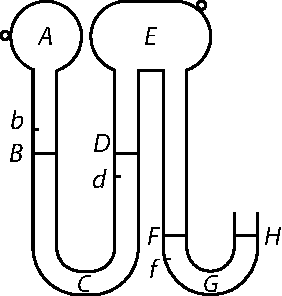
\includegraphics[width=0.20\textwidth]{gesamttex/edit_VIII-4/images/LH_37_04_159_d1_159r.pdf}
\edcaption[0.25em]%
{%
\lbrack\textit{Fig.\:1, gestr.}\rbrack%
}%
\end{edfigure}%
\newpage%
\normalsize%
\vspace*{-0.0em}%
\begin{edfigure}[0.0em][1.5em]%
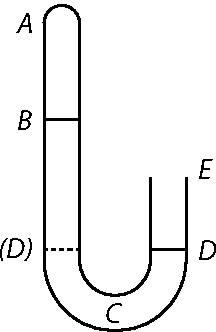
\includegraphics[width=0.19\textwidth]{gesamttex/edit_VIII-4/images/LH_37_04_159_d2_159r.pdf}
\edcaption[0.35em]%
{%
\lbrack\textit{Fig.\:2}\rbrack%
}%
\end{edfigure}%
\pstart%
\noindent%
\edtext{%
Sit Tubus recurvatus%
\indexS{tubus recurvatus}%
}{%
\lemma{Sit}%
\Bfootnote{%
\textit{(1)}~in Tubo %
\textit{(a)}~\textlangle--\textrangle\ %
\textit{(b)}~recurvato %
\textit{(2)}~Tubus recurvatus%
~\textit{L}%
}}
\textit{ABCDE},
Mercurius \textit{BCD}%
\indexS{mercurius in barometro}
ultra horizontem \textit{D}%
\indexS{horizon}%
\edtext{%
\textit{(D)}%
}{%
\lemma{\textit{(D)}}%
\Bfootnote{\textit{erg.\:L}%
}}
eminens,%
\indexS{mercurius eminens ultra horizontem}
quia aer in \textit{AB} rarefactus,%
\indexS{aer rarefactus}%
\indexS{rarefactio aeris}
etsi non omnino nullus,
ajo hinc cognosci posse,
quantum abhinc absit aer,
qui aeque rarefactus%
\indexS{aer rarefactus}%
\indexS{rarefactio aeris}
est %
ac aer \textit{AB}.%
\indexS{aer residuus}
\edtext{%
Nimirum columna aeris%
\indexS{columna aeris}
quae inter ipsum et nos intercedit%
\lbrack,\rbrack%
}{%
\lemma{Nimirum}%
\Bfootnote{%
\textit{(1)}~aer qui intr %
\textit{(2)}~columna aeris %
\lbrack...\rbrack\ nos intercedit%
~\textit{L}%
}}
aequiponderat columnae Mercurii \textit{BD}.%
\indexS{columna mercurii}
Quod sic ostendo%
\lbrack:\rbrack\
auferatur
hinc aer inclusus in \textit{AB},%
\indexS{aer inclusus barometro}
illinc aer supra columnam ei aequiponderantem positus;
patet,
columnam%
\indexS{columna aeris}
et mercurium \textit{B}\textit{(D)}%
\indexS{mercurius in barometro}
sibi aequiponderare,
seu in perfecto aequilibrio%
\indexS{aequilibrium perfectum sive quies}
sive quiete consistere,%
\indexS{quies sive aequilibrium perfectum}
nam nec
\edtext{%
inferiorem aerem magis comprimere,%
\indexS{aer compressus}%
\indexS{compressio aeris}
nec%
}{%
\lemma{inferiorem}%
\Bfootnote{%
\textit{(1)}~comprimere, nec %
\textit{(2)}~aerem magis comprimere, nec%
~\textit{L}%
}}
mercurium%
\indexS{mercurius in barometro}
attollere potest.
Ergo cum tota atmosphaerae columna%
\indexS{columna atmosphaerae}%
\indexS{atmosphaera}
toti aeri \textit{AB}%
\indexS{aer rarefactus}
cum mercurio \textit{BD}%
\indexS{mercurius in barometro}
aequiponderet,
sequitur%
\lbrack:\rbrack\
quod supra columnam
\edtext{%
est,
aequivalere%
}{%
\lemma{est,}%
\Bfootnote{%
\textit{(1)}~aequiponderare %
\textit{(2)}~aequivalere%
~\textit{L}%
}}
aeri \textit{AB}
non pondere tantum,%
\indexS{pondus aeris ambientis}%
\indexS{pondus aeris ordinarii}
sed et
\edtext{%
elaterio,%
\indexS{elaterium aeris ambientis}%
\indexS{elaterium aeris ordinarii}
totam columnam cum Mercurio aequivalente,
quippe mutuo destructis auferendo;%
}{%
\lemma{elaterio,}%
\Bfootnote{%
\textit{(1)}~ponendo enim non totum aerem in %
\textit{(2)}~totam columnam %
\lbrack...\rbrack\ destructis auferendo;%
~\textit{L}%
}}
perinde est,
ac si immediate se tangerent aer ille
immediate supra columnam positus
et aer \textit{AB},
qui non sunt in aequilibrio%
\indexS{aequilibrium in barometro}
nec se
\edtext{%
immutent ex hypothesi,%
\indexS{hypothesis}
nihil enim hic mutatur amplius;
patet
esse e\lbrack ju\rbrack sdem conditionis.%
}{%
\lemma{immutent}%
\Bfootnote{%
\textit{(1)}~patet aerem \textit{AB} esse %
\textit{(2)}~ex hypothesi, %
\lbrack...\rbrack\ amplius; patet %
\textit{(a)}~esse eosdem %
\textit{(b)}~esse \bars{eosdem \textit{ändert Hrsg.}} conditionis.%
~\textit{L}%
}}
Hinc sequitur
aucta \textit{(D)}\textit{B}
\lbrack%
\href{\Scan{LH_37_04_159v}}%
{159\,v\textsuperscript{o}}%
\rbrack\
vel augeri pondus atmosphaerae%
\indexS{pondus atmosphaerae}%
\indexS{atmosphaera}
vel ejus altitudinem,%
\indexS{altitudo atmosphaerae}
scilicet rarefactione aeris inferioris%
\lbrack;\rbrack%
\indexS{rarefactio aeris}%
\indexS{aer rarefactus}
quorum utrum in causa sit,
statim ex duobus collatis Elateriis%
\indexS{elateria aeris collata}
dijudicari potest.
Illud investigandum
an quod ex duobus duci potest,
ex aliis omnibus per consequentiam duci possit,
an vero
pluribus ejusmodi barometris adhibitis%
\indexS{barometrum portabile}%
\indexS{barometrum adhibitum}
plus discamus.
\pend%
\newpage%
\pstart%
Imo video
nihil hic esse
quod non ratiocinando praedici possit,
dato enim gradu rarefactionis aeris%
\indexS{rarefactio aeris}%
\indexS{gradus rarefactionis aeris}%
\indexS{aer rarefactus}
statim praedici potest %
quanta sit virium%
\indexS{vis aeris rarefacti}
\edtext{%
portio.%
\indexS{portio virium}
Verum hoc paulo difficilius est,%
}{%
\lemma{portio}%
\Bfootnote{%
\textit{(1)}~, seu quae usque 
\textit{(2)}~. Verum hoc paulo difficilius est,%
~\textit{L}%
}}
data rarefactione aeris%
\indexS{rarefactio aeris}%
\indexS{aer rarefactus}
in
\edtext{%
\lbrack\textit{AB}\rbrack,%
}{%
\lemma{\textit{ABC}}%
\Bfootnote{%
\textit{L\;ändert Hrsg.}%
}}
invenire
quantus futurus sit ingressus Mercurii%
\indexS{ingressus mercurii}%
\indexS{mercurius in barometro}
seu quanta altitudo \textit{BD}.%
\indexS{altitudo mercurii}
Sed hoc
ni fallor
ita determinabimus.
Aer inclusus%
\indexS{aer inclusus barometro}
\edtext{%
resistit aeri%
\indexS{aer resistens pressioni aeris}%
\indexS{resistentia aeris ad pressionem}%
}{%
\lemma{resistit}%
\Bfootnote{%
\textit{(1)}~Mercurio %
\textit{(2)}~aeri%
~\textit{L}%
}}
posito supra illum
cui pari gradu aequalis
\edtext{%
est%
\lbrack;\rbrack\
columna%
\indexS{columna aeris}
ergo infra%
}{%
\lemma{est}%
\Bfootnote{%
\textit{(1)}~infra %
\textit{(2)}~columna ergo infra%
~\textit{L}%
}}
hunc
tantum in illum aget
cujus vis%
\indexS{vis aeris pressi}
\edtext{%
seu resistentia%
\indexS{resistentia aeris ad pressionem}%
}{%
\lemma{seu resistentia}%
\Bfootnote{%
\textit{erg.\:L}%
}}
nota est;
ob notam hujus densitatem%
\indexS{densitas aeris pressi}
ponatur ea esse \textit{r},
erit
\edtext{%
effectus%
\indexS{effectus pressionis aeris}
ejus in aerem inclusum \textit{r},%
\indexS{aer inclusus barometro}
sed is est duplex%
\lbrack:\rbrack\
unus%
}{%
\lemma{effectus ejus}%
\Bfootnote{%
\textit{(1)}~duplex unus %
\textit{(2)}~in aerem %
\lbrack...\rbrack\ duplex unus%
~\textit{L}%
}}
ut ejus densitas augeatur%
\indexS{densitas aeris pressi}%
\lbrack,\rbrack\
alter
\edtext{%
\lbrack ut\rbrack%
}{%
\lemma{ut}%
\Bfootnote{%
\textit{erg.\;Hrsg.}%
}}
intrudatur
seu sustineatur Mercurius \textit{BCD}.%
\indexS{mercurius intrusus}%
\indexS{mercurius sustentus}
Datur autem quantitas Mercurii%
\indexS{mercurius infusus barometro}
quam infundere volumus
\textit{BCD},
\edtext{%
scilicet
spatium \textit{ABDE} sit \textit{e},
spatium \textit{BCD}
quod Mercurius occupabit%
\indexS{mercurius in barometro}%
\indexS{spatium mercurii in barometro}
sit \textit{m},
erit spatium $AB + DE$ aequ. $e - m$,
et \textit{AB} sit \textit{b}.
Vi\lbrack s\rbrack\ aeris%
}{%
\lemma{scilicet spatium}%
\Bfootnote{%
\textit{(1)}~\textit{AB} est %
\textit{(2)}~\textit{ABCD} sit %
\textit{(a)}~\textit{b}, %
\textit{(b)}~\textit{e}, spatium \textit{BCD} %
\lbrack...\rbrack\ erit spatium %
\textit{(aa)}~\textit{AB} aequ. $b - m$. Ergo ponamus vim %
\textit{(bb)}~$AB + DE$ %
\lbrack...\rbrack\ sit \textit{b}.
\bars{Vim \textit{ändert Hrsg.}} aeris%
~\textit{L}%
}}
per%
\indexS{vis aeris diffusa}
\edtext{%
Totum \textit{ABCD} diffusa ex%
}{%
\lemma{Totum}%
\Bfootnote{%
\textit{(1)}~diffusa ex %
\textit{(2)}~\textit{ABCD} diffusa ex%
~\textit{L}%
}}
hypothesi%
\indexS{hypothesis}
erat \textit{r},
ergo vis ejus inclusi in \textit{AB}%
\indexS{vis aeris inclusi}%
\indexS{aer inclusus barometro}
erit ad diffusam,%
\indexS{vis aeris diffusa}
ut \textit{e} ad
\edtext{%
[\textit{b}],%
}{%
\lemma{$b - m$}%
\Bfootnote{%
\textit{L\;ändert Hrsg.}%
}}
seu in ratione reciproca,%
\indexS{ratio reciproca}
seu erit vis ejus%
\indexS{vis aeris inclusi}%
\indexS{aer inclusus barometro}
\edtext{%
inclusi
$\dfrac{re}{b}$.%
\rule[0.0mm]{0.0mm}{4.2mm}
Sed nondum ideo%
}{%
\lemma{inclusi}%
\Bfootnote{%
\textit{(1)}~$\dfrac{re}{b - m}$ %
\textit{(2)}~$\dfrac{re}{b}$ %
\textit{(a)}~, dato ergo %
\textit{(b)}~. Sed nondum ideo%
~\textit{L}%
}}
scimus punctum \textit{B},
quia nec scimus punctum \textit{D},%
\rule[0.0mm]{0.0mm}{2.8mm}
seu ignoramus
\textit{AB} aequ. \textit{b}
et \textit{DE} aequ. \textit{d},
licet sciamus
$b + d$ aequ. $e - m$.
Ergo una adhuc aequatione%
\indexS{aequatio plana}
opus est,
ut habeatur solutio problematis,%
\indexS{solutio problematis}%
\indexS{problema solvendum}
quam
\edtext{%
ita inveniemus%
\lbrack:\rbrack\
designavimus jam calculo%
\indexS{calculus}
vim inclusi aeris in \textit{AB},%
\indexS{vis aeris inclusi}%
\indexS{aer inclusus barometro}
scilicet
\lbrack$\dfrac{re}{b}$\rbrack,
et possumus quoque designare%
}{%
\lemma{ita}%
\Bfootnote{%
\textit{(1)}~invenimus %
\textit{(2)}~inveniemus %
\textit{(a)}~habemus %
\bars{calculo \textit{erg.}} vim inclusi aeris in \textit{AB}, scilicet $\dfrac{ce}{b}$, habem %
\textit{(b)}~designavimus jam %
\lbrack...\rbrack\ \textit{AB}, scilicet %
\bars{$\dfrac{ce}{b}$ \textit{ändert Hrsg.}} et possumus quoque designare%
~\textit{L}%
}}
vim Mercurii%
\indexS{vis mercurii eminentis supra horizontem}%
\indexS{mercurius eminens supra horizontem}
supra horizontem%
\indexS{horizon}
\edtext{%
eminentis \textit{B}\textit{(D)}
\lbrack quae\rbrack\
ad vim%
}{%
\lemma{eminentis}%
\Bfootnote{%
\textit{(1)}~\textlangle\textit{DB}\textrangle\ %
\textit{(2)}~\textit{B}\textit{(D)} %
\textit{(a)}~s\textlangle c\textrangle\ %
\textit{(b)}~nam %
\textit{(c)}~\bars{quae \textit{erg.\;Hrsg.}} ad vim%
~\textit{L}%
}}
totius Mercurii 27%
\indexS{vis mercurii 27 pollicum}%
\indexS{pollex}
\edtext{%
pollicum,
quam longitudinem vocabimus \textit{l},
est ut \textit{B}\textit{(D)} ad \textit{l}.%
}{%
\lemma{pollicum}%
\Bfootnote{%
\textit{(1)}~quam vocabimus~\textit{v}, %
\textit{(a)}~ut %
\textit{(b)}~est, ut %
\textit{(2)}~quam longitudinem %
\lbrack...\rbrack\ \textit{B}\textit{(D)} ad~\textit{l}.%
~\textit{L}%
}}
Quaerenda ergo
\edtext{%
recta \textit{B}\textit{(D)}
ex datis \textit{e}, \textit{m}%
}{%
\lemma{recta}%
\Bfootnote{%
\textit{(1)}~\textit{AB} ex datis %
\textit{(2)}~\textit{B}\textit{(D)} ex datis \textit{e}, \textit{m}%
~\textit{L}%
}}
et suppositis \textit{b}, \textit{d}.
Nempe datur et \textit{CE}
quam vocabimus \textit{c},
e qua
si detrahatur \textit{ED},
seu \textit{d},
habebitur \textit{CD} aequ. $c - d$,
cujus duplum $2c - 2d$
erit \textit{DC}\textit{(D)},
quae longitudo
si detrahatur a \textit{BCD} seu \textit{m},
tunc restabit \textit{B}\textit{(D)},
ergo erit
$m - 2c - 2d$ aequ.\;\textit{B}\textit{(D)},
\edtext{%
ergo Mercurii \textit{B}\textit{(D)} pondus%
\indexS{pondus mercurii}%
}{%
\lemma{ergo}%
\Bfootnote{%
\textit{(1)}~vis %
\textit{(2)}~Mercurii \textit{B}\textit{(D)} pondus%
~\textit{L}%
}}
erit ad Mercurii in Barometro vacuo pondus \textit{v},%
\indexS{pondus mercurii in barometro vacuo}%
\indexS{mercurius in barometro}%
\indexS{barometrum vacuum}
ut $m - 2c - 2d$ est ad \textit{l}
seu ad 27 pollices circiter,%
\indexS{pondus mercurii 27 pollicum}
ergo pondus Mercurii \textit{B}\textit{(D)} est
$\dfrac{v \smallfrown \overline{m - 2c - 2d}}{l}$.
Quae vis%
\indexS{vis mercurii eminentis supra horizontem}
\ledpb%
addita vi aeris%
\indexS{vis aeris inclusi}
in \textit{AB} inclusi%
\indexS{aer inclusus barometro}
$\dfrac{re}{b}$
aequat vim~\textit{r} totam
quae antea aeri per totum diffuso inerat,%
\indexS{vis aeris diffusa}%
\rule[0.0mm]{0.0mm}{4.6mm}
ergo fiet
$\dfrac{re}{b} + \dfrac{v}{l}\:\overline{m - 2c - 2d}$ aequ. \textit{r},
seu fiet:
$rel + vbm - 2vbc - 2vbd$ aequ. \textit{blr}.%
\rule[0.0mm]{0.0mm}{5.0mm}
Et quia \textit{d} aequ. $e - m - b$,
ideo substituendo eius valorem%
\indexS{valor substituendus}
in priore,
fiet
$rel + \ovalbox{vbm} - 2vbc - 2vbe + {\protect\overset{3}{\ovalbox{2}}} vbm + 2vb^2$
aequ. \textit{blr},%
\rule[0.0mm]{0.0mm}{5.0mm}
quae est aequatio plana,%
\indexS{aequatio plana}
cujus ope facile inveniri potest \textit{b}.
\edtext{%
Quod si aer initio nullo modo fuerit rarefactus,%
\indexS{aer rarefactus}
tunc tantum ponatur \textit{r} aequale \textit{v},%
}{%
\lemma{Quod}%
\Bfootnote{%
\textit{(1)}~si ponatur \textit{r} aequ. \textit{v}, tunc %
\textit{(2)}~si aer %
\lbrack...\rbrack\ aequale \textit{v},%
~\textit{L}%
}}
et fiet
$el - 2bc - 2be + 3bm + b^2$ aequ. \textit{bl},
sublata \textit{l}
\edtext{%
vel \textit{r}.
Tandem notandum%
}{%
\lemma{vel \textit{r}}%
\Bfootnote{%
\textit{(1)}~, seu %
\textit{(2)}~. Quod si in construendo tubo\indexS{tubus construendus} ipsam \textit{c} talem assumsissemus ut esset $-\ 2m- 2e + 3m$ aequ. \textlangle--\textrangle\ %
\textit{(3)}~Tandem notandum%
~\textit{L}%
}}
tam fortem esse aerem initio inclusum \textit{r},%
\indexS{vis aeris inclusi}
et tam debilem Mercurium infusum \textit{d},%
\indexS{vis mercurii infusi}%
\indexS{mercurius infusus barometro}
ut cadat \textit{B} infra horizontem \textit{(D)}.%
\indexS{horizon}
\pend%
\pstart%
Tantum.
\pend%
\selectlanguage{latin}%
\frenchspacing%
\normalsize%
